\documentclass[12pt,journal]{journal}
\usepackage{amsmath}
\usepackage[spanish]{babel} %Definir idioma español
\usepackage[sort&compress]{natbib}
\usepackage[utf8]{inputenc} %Codificacion utf-8

\usepackage{graphicx}
\usepackage{multirow}


\begin{document}

\title{Quantum Network}

\author{Jose~David~Mamani~Vilca}% <-this % stops a space

\onecolumn

\maketitle

\section{Introduction}

A basic definition for Quantum Network is done as follow: \textit{A set of systems, protocols and devices that allows us to create extremely safe connections between computers}. These systems base its functionality using principles of quantum teleportation and qubits. The main difference between this system and traditional networks come in the fact that Quantum Network are only usable in system with the same architecture. 

\section{Some Related Definitions}

\subsubsection{Quantum Network for Computing}

Also called as \textbf{Distributed Quantum Computing}. These systems use the same concept implemented in common Distributed Computing. Using multiple quantum processors in a quantum network and exchanging qubits between them, increase computational power when the whole network works simultaneously \citep{kimble2008quantum} \citep{Caleffi:2018:QIC:3233188.3233224}.


\subsubsection{Quantum Networks for Communication}

Sending qubits from a quantum processor to another over a long distance is the main task required in this kind of network.  This process can be done with local quantum networks connected into a quantum internet. 
Quantum Internet, by the way, is a network of quantum networks that works with the concept of Quantum Entangled Bits (which can be understood as the physical phenomenon that occurs when a pair of particles are generated in a way that its quantum state cannot be describe independently, what means that they are the same even if they are separated by huge distances)
Quantum Internet supports many application requiring very modest quantum processor. Just to figure it out, a protocol of quantum key distribution in quantum cryptography has enough if the quantum processor is able to process only a single qubit at a time. This fact is necessarily required as described because Quantum Entangled Bits works with only two qubits \citep{pednault2017breaking}.


%\begin{figure}[tph!]
%\centerline{\includegraphics[totalheight=7cm]{draw_1}}
%	\centering
%    \caption{Tiempo de Insercción en relación al número de threads}
%\end{figure} 


\section{Elements of a Quantum Network}

A Quantum Network can be described in the same way as traditional Networks are.

\begin{itemize}

\item First, we have end nodes that are used in the application layer. These nodes are composed by different quantum processors of a least one qubit. Of course, we can find quantum processors which accept several qubits, but those cases are not very common due to the fact that those systems in which are used requires much more memory. 

\item Second, we find something related to the transportation of qubits. This is referred as communication and is done using standard telecommunication optical fibers and photo-based qubits. If the quantum processors are very close each other, different wavelengths can be used taking in account the exact hardware platform of the quantum processor.

\item Third. Even if we have the transportation layer, we cannot use it without something capable of \textit{formatting} and delivering the qubit to the intended quantum processor. To do so, we require the use of optical switches which can preserve the quantum coherence, something that can be really challenging.

\item Finally, and maybe, the most important part is defined as Trusted Repeaters and Quantum Repeater. These devices are completely different from its analogous in traditional network but they got the same functionality. A trusted repeater appears between end nodes \citep{van2014quantum} and takes the responsibility of \textit{duplicate} a qubit so that this can reach its destination. A trusted repeater can only be used to perform quantum key distribution.

At this point, is important to know that a qubit cannot be replicated, so the functionality of these devices could be a little confusing.
So, let is explain this functionality with an example:

\begin{enumerate}
\item A Trusted Repeater is established between Alice and Bob (because they live far away from each other). When Alice sends a polarized photon to Bob (A qubit with a defined value), the Trusted Repeater will receive it instead of Bob.

\item It is impossible to copy the state of a photon without knowing it, so the Trusted Repeater will measure the polarization of each photon. 

\item Once the Trusted Repeater have the needed information, it will rebuild a new photon and send it to Bob. Obviously, this photon will be the same that Alice sent at the beginning (At least in its state). 

\end{enumerate}

Doing this, we can increase the cast range when we send qubits. 

In the other side, a Quantum Repeater allows the end to end generation of quantum entanglement using quantum teleportation. This means that communication can be established between distant nodes without physically sending the qubit the entire distance \citep{bouwmeester1997experimental}.


\begin{figure}[tph!]
\centerline{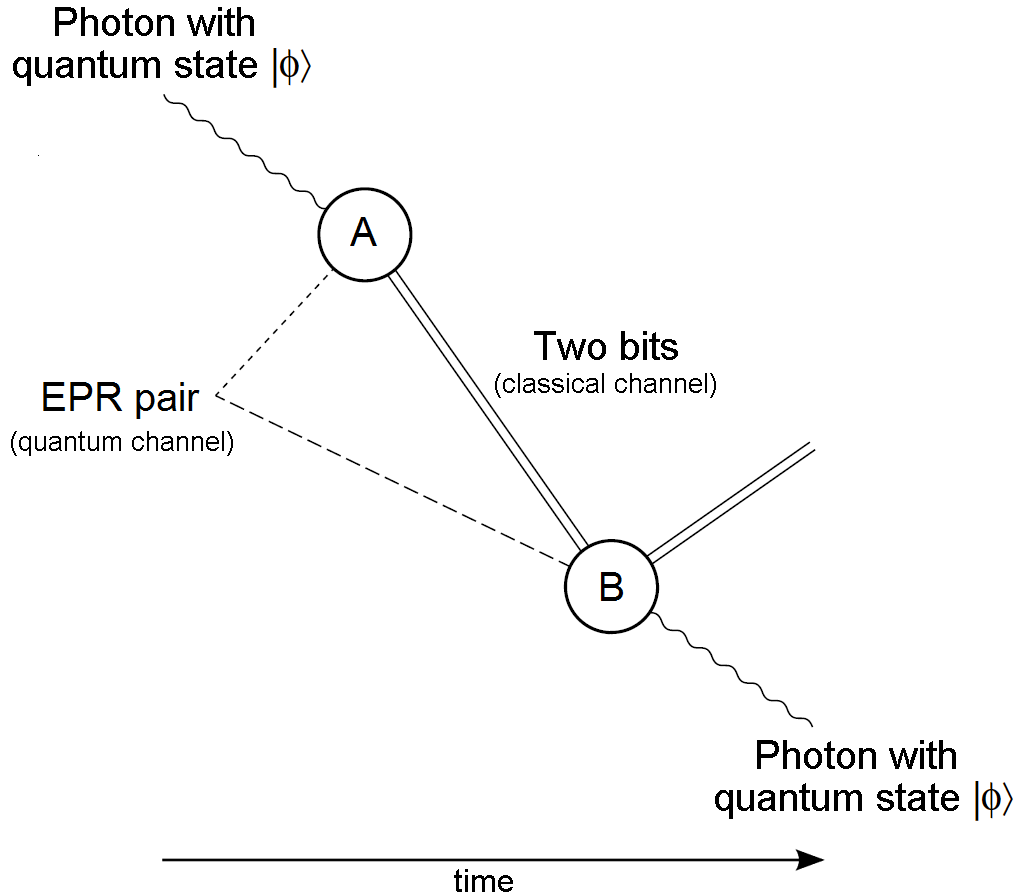
\includegraphics[totalheight=6cm]{1}}
	\centering
    \caption{Photon teleportation diagram}
\end{figure}

For example, having two pairs of entangled qubits $[A, Ra]$ and $[Rb, B]$ where $[A]$ is the sender $[Ra, Rb]$ the Repeater and $[B]$ the receiver. The initial entangled bits can easily be established using, for example, parametric down conversion. Then, the teleportation can be done first between A and Ra, and after between Rb and B.  To go from Ra to Rb a process called Bell Measurement is required.


With this implementation we simulate a teleportation between A and B.


\end{itemize}



\section{Some applications}

\subsection{Secure Communications}

One of the most important features required in communication is privacy \citep{metwaly2015architecture}. For Quantum Communication, this task can be done with impressive guarantee.  Applying a quantum operator defined by the user, a message can be sent without chances of eavesdropping. This come from the fact that if a listener tries to catch the messages, the information will be modified and the intruder will be detected. Furthermore, if the intruder does not know the quantum operator, information will get corrupted \citep{wiki:xxx}.

\subsection{Jamming}

Jamming can be defined as an attack where the intruder will get the information that was not intended for him and, in some cases, stop the real proper from receiving the messages.  This kind of attack can be avoided in Quantum Networks using algorithms of Frequency-Hopping Spread Spectrum. Basically, the sender and the receiver will iterate in random frequencies defined by the algorithm with the condition that will be the same at any time. This method can also be improved adding a quantum operator, a concept previously defined \citep{wiki:xxx}.

\bibliographystyle{abbrv}
\bibliography{biblio} 


 
\end{document}